\documentclass[border=4pt]{standalone}
\usepackage{tikz}
\usetikzlibrary{positioning, arrows.meta, shapes.geometric, calc, fit, backgrounds}
\usepackage{amsmath,amssymb}
\begin{document}
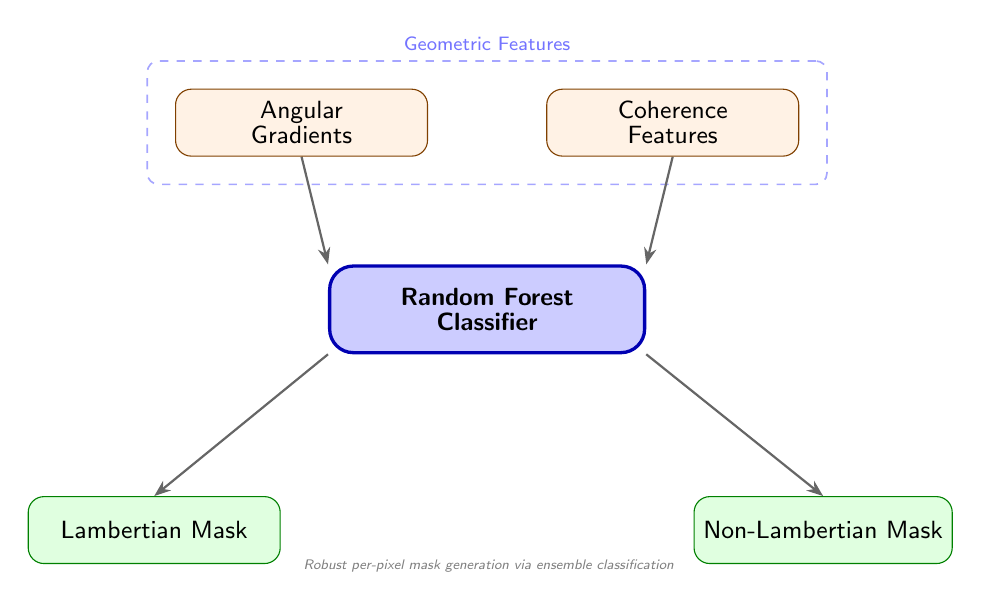
\begin{tikzpicture}[
  feature/.style={draw, rounded corners=2mm, minimum width=3.2cm, minimum height=0.85cm,
                  fill=orange!10, draw=orange!50!black, align=center,
                  font=\sffamily\small},
  innov/.style={draw, rounded corners=3mm, minimum width=4.0cm, minimum height=1.1cm,
                fill=blue!20, draw=blue!70!black, line width=1.2pt, align=center,
                font=\sffamily\small\bfseries},
  output/.style={draw, rounded corners=2mm, minimum width=3.2cm, minimum height=0.85cm,
                 fill=green!12, draw=green!50!black, align=center,
                 font=\sffamily\small},
  arr/.style={-{Stealth[length=6pt]}, thick, color=black!60},
  lbl/.style={font=\sffamily\scriptsize, text=black!45, fill=white, inner sep=1pt},
  gbox/.style={draw=blue!35, dashed, rounded corners=4pt, inner sep=10pt,
               line width=0.6pt},
  annot/.style={font=\sffamily\tiny\itshape, text=black!50},
]

% ---- Feature inputs (top row) ----
\node[feature] (m1) {Angular\\[-2pt]Gradients};
\node[feature, right=1.5cm of m1] (m2) {Coherence\\[-2pt]Features};

% ---- Classifier (center, innovation) ----
\node[innov, below=1.8cm of $(m1)!0.5!(m2)$] (m3) {Random Forest\\[-2pt]Classifier};

% ---- Output masks (bottom row) ----
\node[output, below left=1.8cm and 0.6cm of m3] (m4) {Lambertian Mask};
\node[output, below right=1.8cm and 0.6cm of m3] (m5) {Non-Lambertian Mask};

% ---- Group box for features ----
\begin{scope}[on background layer]
  \node[gbox, fit=(m1)(m2),
        label={[font=\sffamily\scriptsize, text=blue!55]above:Geometric Features}] (g1) {};
\end{scope}

% ---- Arrows (drawn on background to avoid overlap) ----
\begin{scope}[on background layer]
  % Features -> Classifier
  \draw[arr] (m1.south) -- (m3.north west);
  \draw[arr] (m2.south) -- (m3.north east);

  % Classifier -> Masks
  \draw[arr] (m3.south west) -- (m4.north);
  \draw[arr] (m3.south east) -- (m5.north);
\end{scope}

% ---- Annotation ----
\node[annot, below=0.25cm of $(m4)!0.5!(m5)$] {Robust per-pixel mask generation via ensemble classification};

\end{tikzpicture}
\end{document}